\documentclass[11pt,a4paper]{article}
\usepackage[margin=2.4cm]{geometry}
\usepackage[T1]{fontenc}
\usepackage{booktabs}
\usepackage[font=small,labelformat=empty,skip=4pt]{caption}
\usepackage{array}
\usepackage{xcolor}
\usepackage{titlesec}
\usepackage{enumitem}
\usepackage{tcolorbox}
\tcbuselibrary{breakable}
\usepackage{tikz}
\usetikzlibrary{arrows.meta,positioning,calc}
\usepackage{graphicx}
\usepackage[hidelinks]{hyperref}

\definecolor{good}{HTML}{1B7F3B}
\definecolor{warn}{HTML}{B26B00}
\definecolor{bad}{HTML}{B3261E}
\definecolor{grey}{HTML}{666666}
\definecolor{rule}{HTML}{2B4C7E}

\newcommand{\code}[1]{\texttt{#1}}
\newcommand{\dn}{\textcolor{good}{\textbf{done}}}
\newcommand{\fl}{\textcolor{warn}{\textbf{in flight}}}
\newcommand{\ns}{\textcolor{grey}{not started}}
\newcommand{\done}{\textcolor{good}{\textbf{DONE}}}
\newcommand{\prog}{\textcolor{warn}{\textbf{IN PROGRESS}}}
\newcommand{\todo}{\textcolor{grey}{\textbf{NOT STARTED}}}
\newcommand{\stopp}{\textcolor{bad!30!white}{\textbf{STOP}}}
\newcommand{\solid}{\textcolor{good}{\textbf{solid}}}
\newcommand{\weak}{\textcolor{warn}{\textbf{weak}}}
\newcommand{\unsup}{\textcolor{bad}{\textbf{unsupported}}}

\titleformat{\section}{\large\bfseries\color{rule}}{\thesection.}{0.6em}{}
\titleformat{\subsection}{\normalsize\bfseries}{}{0em}{}
\setlist[itemize]{leftmargin=1.1em,itemsep=2pt,topsep=3pt}
\setlength{\parskip}{5pt}
\setlength{\parindent}{0pt}
\renewcommand{\arraystretch}{1.25}

\newtcolorbox{phasebox}[1]{breakable,colback=white,colframe=rule!55,boxrule=0.7pt,
  arc=2pt,left=8pt,right=8pt,top=6pt,bottom=6pt,title={\bfseries #1},
  fonttitle=\color{white},colbacktitle=rule}

\newtcolorbox{stopbox}{breakable,colback=bad!3,colframe=bad!55,boxrule=0.7pt,
  arc=2pt,left=8pt,right=8pt,top=5pt,bottom=5pt}

\title{\textbf{Plexus Discovery --- Cardiomyocytes}\\[6pt]
\large Progress note --- written to be read, not decoded}
\author{}
\date{2 August 2026}

\begin{document}
\maketitle
\vspace{-2.2\baselineskip}

\begin{center}\small\color{grey}
The third loop, and the first one pointed at a real measurement rather than a paper.\\
Plain English throughout. Organised by phase, because phases are where we stop and you decide.
\end{center}

\vspace{4pt}
\hrule
\vspace{10pt}

%======================================================================
\section{What we are doing --- two things at once}

\textbf{Track A --- build the method.} The same automated loop as the Okuda folder: it proposes a
change to the \emph{mechanism}, writes down what it expects before running, runs, measures, and
records whether it was right. One thing here is new and it changes the machine. In the Okuda loop a
run is a simulation that is then scored. Here a run is a \emph{fit}: the simulation is
differentiable, so the computer can be told ``make this match the recording'' and it will adjust the
model until it does. That is a far stronger instrument and a far more dangerous one, and most of the
pre-flight work below exists because of the second half of that sentence.

\textbf{Track B --- reproduce the beating tissue, as the proof that Track A works.} We have a
microscope recording of a sheet of human heart-muscle cells contracting on a soft gel, and one of a
diseased sheet from a patient with a thickened heart muscle. The target is no longer a picture from
someone's paper --- it is a measurement, with error bars we can compute ourselves. \emph{The
reproduction is the evidence.}

The two tracks feed each other exactly as before: the reproduction is the honest test of the method,
and the method is what makes the reproduction more than curve-fitting.

%======================================================================
\section{Where we actually are}

\textbf{Nothing is believed. That is a decision, not an accident.} A previous, single-agent campaign
ran sixty rounds on this data and produced a confident ledger of established mechanisms. We are
keeping none of it. The reason is not that its conclusions were foolish --- it is that they were
reached with rulers nobody had checked, on a fit that was never once tested against data it had not
already seen, in a program that never fixed its random number generator. A conclusion drawn that way
cannot be repaired by re-reading it; it can only be re-earned.

\textbf{But nothing is thrown away either.} Every claim that campaign made is transcribed into a
register of \emph{open questions}, each stamped \emph{untested}, and a second register of things we
believe is created \textbf{with zero entries in it}. That is the difference between discarding
sixty rounds of work and discarding sixty rounds of unearned confidence. \emph{Some of those
hypotheses are probably right, and we will find out which in the ordinary way.}

\textbf{This includes the settings.} A default is a belief in disguise: one option in the old
trainer still defaults to a path chosen because a retired ledger called the alternative harmful, and
the reason is written into the help text. Defaults go into the register of open questions along with
everything else.

\textbf{Two facts about today, both measured this morning.} The training program does not run at
all --- it stops immediately with a missing-function error, so the sixty-first round could not have
happened even if we had wanted it. And the simulation, as the Plexus library currently stands, is
\emph{not} differentiable: ask it for a gradient through a specification file and it returns
nothing. The old program worked only by going around the library rather than through it. Both are
fixable, both have a phase below, and both are much better to know now.

%======================================================================
\section{The loop, in four steps}

The Okuda loop has thirteen roles. That is the right answer to a search over model \emph{structure}
with no data to appeal to. It is the wrong answer here, and the shape of this loop was settled by
one instruction: \textbf{make it brutally concrete.}

\begin{center}
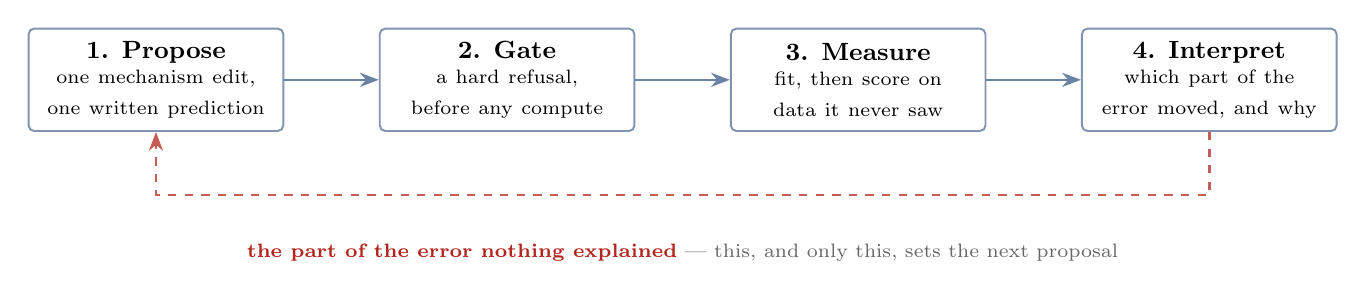
\begin{tikzpicture}[
  box/.style={draw=rule!60,fill=white,rounded corners=2pt,line width=0.7pt,
              minimum height=13mm,text width=30mm,align=center,font=\small},
  lbl/.style={font=\scriptsize\color{grey},align=center},
  ar/.style={-{Stealth[length=2.4mm]},line width=0.8pt,draw=rule!70},
  fb/.style={-{Stealth[length=2.4mm]},line width=0.9pt,draw=bad!75,dashed}]
\node[box] (p) {\textbf{1. Propose}\\[1pt]\scriptsize one mechanism edit,\\one written prediction};
\node[box,right=12mm of p] (g) {\textbf{2. Gate}\\[1pt]\scriptsize a hard refusal,\\before any compute};
\node[box,right=12mm of g] (m) {\textbf{3. Measure}\\[1pt]\scriptsize fit, then score on\\data it never saw};
\node[box,right=12mm of m] (i) {\textbf{4. Interpret}\\[1pt]\scriptsize which part of the\\error moved, and why};
\draw[ar] (p) -- (g);
\draw[ar] (g) -- (m);
\draw[ar] (m) -- (i);
\draw[fb] (i.south) -- ++(0,-8mm) -| (p.south);
\node[lbl,below=13mm of g.south east,xshift=6mm]
  {\textbf{\color{bad}the part of the error nothing explained} --- this, and only this, sets the next proposal};
\end{tikzpicture}
\end{center}

\textbf{Step 1 --- Propose.} One change to the mechanism, and one sentence saying what it will do,
containing a number that could turn out to be wrong. Not ``this should improve the fit''.

\textbf{Step 2 --- Gate.} A deterministic refusal, spent before a second of compute. Does it run? Is
the prediction one that could fail? Is the quantity it names one we have proved we can measure? Is
the effect it predicts bigger than the noise? Is there a control? \textbf{The gate is code and it
cannot be argued with.} Nearly every wasted week of the previous campaign was a run this gate would
have refused for free.

\textbf{Step 3 --- Measure, on the real series.} The fit happens, and then the model is scored
\emph{against frames it was not fitted to}. The output is not a score; it is a \emph{decomposition
of the error} --- how much of the mismatch is size, how much is shape, how much is timing, and how
much is in a place the model has no name for.

\textbf{Step 4 --- Interpret.} Which component of that error moved, was the prediction right, and
--- the only question that finally matters --- \emph{what is left that nothing accounts for}.

\textbf{And then the edge that closes the cycle.} That unexplained remainder is the input to the next
proposal. If no mechanism we already have can address it, the loop is not permitted to shrug: it
must say so, and ask for a new one. \textbf{A loop that cannot explain its residual, and cannot say
what would, has stopped doing science and started tuning.} This is the whole design.

\textbf{One hazard this loop has that the Okuda loop does not.} With gradients, adding freedom to a
model almost always improves the fit, and means nothing. So every proposed mechanism is run twice:
once as itself, and once as a \emph{capacity-matched control} --- the same number of new free
numbers, arranged so they cannot mean anything. A mechanism that does not beat its own sham is not a
mechanism.

%======================================================================
\section{What the recording can and cannot support}

This section did not exist in the Okuda note and it is the most important one here. Okuda's target
was a drawing in a paper; ours is a measurement, and a measurement has limits that can be computed
before you start. Everything below was measured from the files this morning.

\textbf{What we have --- two specimens, under five filenames.} One healthy sheet and one diseased
sheet, filmed on the same rig. They appear on disk as five different files, because each was tracked
more than once: the healthy one twice, the diseased one three times, under names that do not say so.
Two of those files looked like independent replicates and are not --- they are crops of the same two
movies. \textbf{So the dataset is one healthy specimen and one diseased specimen, and that is the
hard ceiling of the enterprise.} It is also why the held-out specimen will be sealed by what it
contains rather than by where it lives: sealing a filename would seal nothing.

It is a confluent \emph{sheet}, not a single cell --- there is no isolated contracting object in the
field of view --- so the unit that could be replicated is the well, and we have one of each. No
statistic may be computed over the tracked points as though they were independent samples.

The healthy recording is 239 frames at 24 frames a second --- just under ten seconds --- of a grid
of 18{,}769 tracked points. Five contractions, four complete cycles, one every 2.1 seconds. The
motion is tiny: a typical point moves about 4 pixels and the largest about 15, on a 2048-pixel
image.

\textbf{The clock is trustworthy; the map is not.} Between beats the tissue is still and the
frame-to-frame jitter is 0.017 pixels --- the beat is 155 times larger, and four independent
estimators agree. But that is noise \emph{in time}. In space the same quiet field is essentially
structureless at the smallest scale, and two independent trackings of the same movie disagree about
the pattern almost completely (below). \textbf{When the beat happens, and how strong it is, are
solid measurements. Where it happens, in fine detail, is not.}

\textbf{The information content is the problem.} Written as a set of spatial patterns, the beat is
\textbf{90\% one pattern and 99\% three patterns}. The whole recording holds roughly a hundred
independent patches of information. The previous fit gave itself two freely-shaped fields of about
two hundred thousand numbers each to describe it. \emph{That is not a fit, it is an interpolation},
and no amount of good behaviour by the optimiser makes it otherwise. How big the model is allowed to
be therefore becomes a measured quantity, not a habit.

\textbf{A held-out beat is not a real test --- and it sets a bar nothing has cleared.} We measured
it rather than assuming it: predict any one beat from the average of the other three and you already
score 0.98. The beats are near-copies, so ``it generalises to the next beat'' would be a claim about
almost nothing. \textbf{The only genuine held-out specimen is the diseased sheet}, and we verified
it loads with no code changes at all.

But the same fact has a much sharper edge, and it is the single most important number in this note.
\emph{Simply copying the previous beat} --- no model, no physics, no fitting --- \textbf{scores
higher on both available measures than the best of the 324 fits the previous campaign ever
produced.} That is the bar. Any mechanism we propose has to beat the cheapest imaginable
alternative, and nothing yet has.

\textbf{The most serious finding, and it constrains what we may ever claim.} The same movie was
independently tracked twice. The two trackings agree almost perfectly on \emph{when} and \emph{how
much} the tissue moves --- their beat-by-beat time courses match at 0.998. They disagree on
\emph{where}: the two displacement maps correlate at 0.12 and 0.28. In plain terms, \textbf{the
rhythm and the strength of the beat are reproducible facts about the tissue; the fine spatial pattern
is substantially a property of the tracking software.} A campaign whose product is a learned map of
stiffness across the sheet would be measuring the tracker. Phase~1 pins this number down properly,
and it may well redirect the programme toward claims about the whole cell rather than about places
inside it.

\textbf{Three limits from our own simulation rather than the data.} The real motion is smaller than
one cell of the simulation grid --- two-thirds of one cell at the peak of the beat --- so the
simulation's internal smoothing is coarser than the thing being measured, and the numerical method
may be doing the modelling. The model also carries fewer particles than the recording has tracked
points, on a coarser grid, so there is a ceiling on how much of the measurement it could reproduce
even in principle; that ceiling should be measured and printed beside the data's own. And the grid
size, the particle count and the number of sub-steps were all inherited and never once tested. All
three are settled by running finer and checking the answer stops moving.

\textbf{And one limit that is nobody's fault.} There is a single substrate stiffness, no drug, and
no change of pacing --- one condition, one observable, no perturbation. A mechanics model tested
against a single unperturbed recording can be made to fit; it cannot really be challenged. Worth
knowing now, because the cheapest fix is not more computing, it is asking the Utrecht group for
another condition.

%======================================================================
\section{What we are not carrying forward, and why}

Four measurements from the audit make the case on their own. None of them is about biology.

\footnotesize
\begin{tabular}{@{}l p{11.2cm}@{}}
\toprule
\textbf{what} & \textbf{what was measured}\\
\midrule
the dice were never fixed & No random seed was ever set. Two runs of the \emph{same command}, with
no training at all, differ by 83\% of the size of the signal being fitted. Fix the seed and they
agree to seven decimal places. Rankings in the old record were decided on differences of 0.003.\\
the rulers had no zero & A model that predicts \emph{no motion at all} does not score zero on the
measure everything was ranked by --- it scores $+0.075$, with a spread of $\pm 0.117$, while the
code's own documentation says a do-nothing model scores zero. On the second, older measure the same
do-nothing model scores $-0.875$ and \textbf{the best fit in the whole archive scores $-0.912$},
which is worse. Neither number was ever read against its own null, so neither could say whether
anything had been achieved.\\
the ruler cannot see the
one thing that matters & Give every one of the 18{,}769 points its own random timing offset --- destroy
the coordination completely, so that no two points contract together --- and the measure everything
was ranked by returns \textbf{a perfect score}. It is exactly blind to whether the tissue beats as
one, which is the defining property of heart muscle. Several of the mechanisms the campaign
proposed, argued about and retired were about coordination, and could never have been scored.\\
nothing was ever held out & Sixty rounds fitted one beat of one specimen and scored the same beat of
the same specimen. The diseased sheet was on disk the whole time and was never opened.\\
\bottomrule
\end{tabular}
\normalsize

\textbf{One accusation withdrawn, and a different one raised in its place.} It was reasonable to
worry that the fit was cheating through its edges: a band around the sheet --- 31\% of it --- is
pinned to the real recording every frame, so part of the answer is handed over. We tested it
directly by switching the muscle off and asking how much of the interior still moves. \textbf{The
answer is exactly none} --- not ``a little'', but bit-for-bit zero. So the pinned edge is not
secretly driving the fit. It is, however, still pinned \emph{while the score is being computed},
which means ``held-out'' is not yet a defined term in this apparatus. Every claim will therefore
carry a second column: the same score with the edge released and the model left to run free. And an
edge that transmits nothing inward raises its own question --- what is it for? --- which the
anchoring ladder in Phase~2 answers.

\textbf{Kept, on probation: the apparatus.} The ingested recording; the trainer's hand-rolled
simulation loop; the error-decomposition code; the cluster machinery, which is genuinely
battle-hardened. From the Okuda folder, the deterministic parts port almost unchanged --- the
prediction scorer, the claim register, the record-builder, the cluster driver. And two pieces of
existing Plexus machinery are exactly what this loop needs: the gradient auditor in
\code{operators/diff/}, which already classifies whether a given knob is genuinely learnable, and
the fitting harness from the jax-morph atlas.

\textbf{One inheritance that has to be actively removed.} The old conclusions are compiled into the
source as comments, help strings and defaults. Any agent that reads the trainer inherits the retired
ledger whether we like it or not. Deleting those is a Phase~0 item and it is not cosmetic.

%======================================================================
\section{The team, mapped onto the four steps}

The rule from the Okuda rebuild carries over unchanged: \textbf{a role exists only where it adds
information that is not already available}, and where a question has a deterministic answer, code
answers it. Every role has to earn its place inside one of the four steps or be dropped.

\begin{center}\small
\begin{tabular}{@{}l l p{7.5cm} l@{}}
\toprule
\textbf{step} & \textbf{who} & \textbf{what it adds that nothing else has} & \textbf{kind}\\
\midrule
1 Propose & Proposer & the next mechanism edit, and the prediction it is willing to be wrong about
& agent\\
1 Propose & Peer-review & is this prediction one that could actually fail? Advises, cannot refuse
& agent\\
\midrule
2 Gate & Critic & can it run: legal edit, operator resolves, seed set, control present, not already
done, capacity within the honest size. \textbf{Refuses} & \textbf{code}\\
2 Gate & Physiologist & could this be a heart cell: rhythm, strain, no net drift, nothing leaving the
dish. Reads the premise list rather than restating it. \textbf{Refuses} & \textbf{code}\\
2 Gate & Metrologist & is the named quantity certified, used inside its declared range, and is the
predicted effect \emph{bigger than the noise floor}? \textbf{Refuses} & \textbf{code}\\
\midrule
3 Measure & the fit & the expensive step: optimise, then score with the edge released, on frames it
never saw & \textbf{code}\\
3 Measure & Convergence & did the optimiser finish, or are we reading a half-trained model? An
unfinished fit is a fact about the optimiser, not about the tissue & \textbf{code}\\
3 Measure & Identifiability & \emph{could this mechanism ever have been seen in this recording?}
From the gradients directly. Impossible without differentiability, and the thing we most lacked
& \textbf{code}\\
3 Measure & Replicator & the same thing several times, so that ``different'' has a meaning
& \textbf{code}\\
3 Measure & Collector & builds the round's record from the files on disk. A \code{for} loop, never
an agent, because an agent that collects can forget silently & \textbf{code}\\
\midrule
4 Interpret & Reader & what happened in this run, from the pictures: it labels, it does not measure
& agent\\
4 Interpret & Interpreter & the causal account, and the naming of what is left unexplained & agent\\
4 Interpret & \code{predict.py} & was the prediction right? \textbf{Arithmetic. No agent decides
this} & \textbf{code}\\
\midrule
close & Escalation & the residual nothing explains becomes a written request for a new mechanism
& agent\\
close & Supervisor & what runs next and how much of it; owns the budget & \textbf{code}\\
\bottomrule
\end{tabular}
\end{center}

\textbf{Five agents, nine deterministic checks.} Against the Okuda roster the Grounder goes --- there
is no paper to ground, the data is the ground; the Eye-check folds into the Reader; the
Diagnostician's job shrinks, because a fit that fails fails loudly; and the Archivist waits until
there is a history worth having one for. \textbf{Three roles are new, and all three exist only
because the model is differentiable}: Identifiability, Convergence and the Replicator.

\textbf{Why Identifiability is the important addition.} The previous campaign's final conclusion was
that a whole family of mechanisms was inert --- push harder, damp more, twist more, nothing changed
--- so the limit must be structural. Every one of those was a flat line read by eye with no error
bar. A flat line has three completely different causes: the effect is smaller than the noise, the
recording cannot resolve the mechanism at all, or the response really is flat. The old record fused
all three into one phrase. \textbf{Gradients separate them in a single backward pass}, and the
sentence changes from a law of nature into a statement about the experiment: \emph{this recording
cannot distinguish that mechanism, and here is what would.}

%======================================================================
\section{The phases}

Five stages before the loop is allowed to run, then the loop. \textbf{I stop at the end of each one
and wait for you.} That is the partition, and it is the same ladder as the other two folders.

The rule that ordered them is the one the Okuda folder learned the expensive way: \emph{no
experiment until every instrument it will be read with exists and has been proved to work.} Over
there, three batteries of runs were launched and thrown away because a ruler turned out to be
broken. Here we already know the rulers are broken, so there is no excuse.

\textbf{Two of the gates below are stops, not gates}, and they can end the project. They are marked.
Everything else may be renegotiated if it runs over budget --- \textbf{those two may not}, because a
gate with a waiver attached is not a gate, and a stop that can be waived would be waived at exactly
the moment it was doing its job.

\begin{phasebox}{Phase 0 --- Make it run, make it repeat, publish the empty register \hfill \dn\ (18 of 18)}
\textbf{Goal.} Get from ``nothing executes'' to ``the same command twice gives the same answer, and
we can say exactly what we believe''. None of this is science; each item makes a question askable.

\begin{itemize}
\item \textbf{Repair the apparatus.} The trainer dies on every invocation on a function one branch
deleted from under another. Two of the plotting tools die on a module that no longer exists.
\item \textbf{Fix the dice.} A seed, wired into everything that draws a random number, plus
deterministic arithmetic on the GPU --- and then \emph{two} noise measurements, because they are
different: the spread across seeds, and the spread of the very same seed run twice, which is not
zero unless determinism is forced.
\item \textbf{One path to the data, no fallbacks.} The loader currently tries three locations and
uses whichever exists, so a fit against the wrong recording would never announce itself. One
explicit path; a missing file is a hard error naming what it wanted.
\item \textbf{A run must be recoverable from its own folder.} Commit, full command line, and a
checksum of every input written beside every number --- and if the working tree is dirty, the
differences are written in too. Two batches of the previous campaign were lost to a branch switch;
the cure is not tidiness, it is that the artefact carries its own provenance.
\item \textbf{Publish the two registers.} Every claim of the sixty rounds transcribed as an open
question marked \emph{untested} --- including the ones hiding as defaults. And the register of
things we believe, created with nothing in it.
\item \textbf{Re-check the audit itself.} The list of pitfalls in this note is a claim like any
other. Each item gets a mechanical check. \emph{One has already failed}: a mechanism the old log
recorded as lost is present in the tree after all. It goes into the open questions with everything
else.
\end{itemize}

\textbf{Exit gate.} The trainer runs a short fit end to end; two runs at one seed agree bitwise;
the recording rebuilds from committed code and matches the existing file exactly; a search of the
source for the retired conclusions returns nothing; the register of beliefs has zero entries; and
\textbf{the certification script, run in canary mode, injects six faults and refuses all six.}
A gate that has never been seen to refuse is not a gate.

\textbf{Cost.} About half a day, no GPU.
\end{phasebox}

\begin{phasebox}{Phase 1 --- Freeze the recording, seal the test \hfill \todo}
\textbf{Goal.} Decide, once and in writing, what a run is allowed to see --- \emph{before} anything
is fitted. A split invented later is a split negotiated with the result already in hand.

\begin{itemize}
\item \textbf{The beat inventory}, from the files: onsets, periods, which beats are complete, and
which stretch at the end is not a beat at all and must not be treated as one.
\item \textbf{The ceiling the data sets on itself.} Score each real beat against each other real
beat. \textbf{No model may be scored better than the data agrees with itself}, and that number goes
on the front page of everything afterwards.
\item \textbf{How much of the pattern is the tracker.} The healthy sheet was tracked twice, the
diseased sheet three times. Comparing one tracking against another is the cleanest measurement of
what part of the spatial detail belongs to the tissue. \textbf{This is the number that decides
whether learned maps across the sheet are a legitimate product of this project.}
\item \textbf{Does the answer depend on the grid?} Run at finer resolutions, more particles, smaller
sub-steps. The real motion is smaller than one grid cell, so this is not a formality.
\item \textbf{Freeze the split, and seal the diseased sheet.} Fit frames, held-out frames, held-out
specimen, written down and checksummed. The seal is \textbf{by content, not by filename} --- the
same diseased recording sits on disk under three different names, and sealing one path would seal
nothing. A
run that touches sealed data aborts, and every read of it is logged.
\end{itemize}

\textbf{Exit gate.} The split file exists with disjoint frame sets and the sealed checksums; the
self-agreement number and the tracker-reproducibility number are measured and written into this note;
the resolution check is reported as a number against the noise floor; and a test proves that a run
reading the sealed specimen aborts.

\textbf{Cost.} About a day, no GPU.
\end{phasebox}

\begin{phasebox}{Phase 2 --- Certify the ruler, and find the floor \hfill \todo\ \ \stopp}
\textbf{Goal.} Every number the loop ranks on must have a proved zero, a proved noise level, and a
demonstrated ability to be wrong. \emph{A measure whose null and whose spread are unknown cannot
support a finding, and the previous campaign is sixty rounds of proof.}

\begin{itemize}
\item \textbf{Where is zero?} Score the trivial models: predict no motion; predict the average
motion; \textbf{copy the previous beat}; interpolate inward from the pinned edge with no physics at
all; run the same model with the muscle switched off; and run it with the fields present but never
trained, because \emph{freezing a field is not the same as removing it}. Every score afterwards is
reported as a \textbf{difference from that floor} --- never as a bare number, never as a ratio,
because both can be made to look like anything when the floor is not at zero.
\item \textbf{Teach the ruler to see coordination.} The current measure returns a perfect score for a
sheet whose points beat in completely random order. Until a measure exists that can tell a
coordinated contraction from an incoherent one, no mechanism about timing, waves or rotation can be
proposed, tested or refuted --- and the gate must say so rather than scoring them anyway.
\item \textbf{Is the model even in the right regime?} The trainer's own comments say the loop shape
it rewards comes from \emph{inertial recoil} --- a sheet of cells on a soft gel is overwhelmingly
dominated by drag instead. Set the mass to zero and see whether the effect survives. If it does not,
the objective's favourite feature is an artefact of a regime the tissue is not in.
\item \textbf{How big is nothing?} The same configuration, several seeds, at the depth the loop will
actually use. That spread becomes \textbf{the unit of the whole campaign}: a difference smaller than
it is reported as \emph{indistinguishable} and the gate refuses to let anyone call it a finding.
\item \textbf{Does the ruler measure what it claims?} Take the real recording and distort it one way
at a time --- bigger, rounder, rotated, delayed, shifted --- and confirm the measure moves when it
should and does not move when it should not. Tests that merely restate the documentation do not
count; the documentation is already wrong about where zero is.
\item \textbf{Fix the defects already found in it.} The scoring window is 53 frames for a 50-frame
heartbeat, so it is being asked to close a loop it has over-run; motion is measured from a frame
that sits in the middle of a contraction rather than at rest; one weighting is hard-coded where it
should be declared.
\item \textbf{The anchoring ladder.} Vary the pinned band from nothing to wide, scoring on \emph{one
frozen set of nodes} so the model changes and the ruler does not, and publish what the edge is worth.
The operating width is then chosen on stability --- of the \emph{active} model --- never on score,
because choosing it on score is how the anchor gets tuned until the model wins.
\item \textbf{Build the error decomposition properly.} Step 3 of the loop must return \emph{where}
the model is wrong, in named parts that add up: size, shape, orientation, timing, remainder. The
remainder drives the next round, so it has to be real.
\end{itemize}

\begin{stopbox}
\textbf{THE STOP.} At the end of this phase we know whether the active model beats \emph{the best of
the trivial alternatives} by more than the noise --- and the comparison, the aggregation rule and
the margin are written into code \emph{before} the numbers exist, so that the verdict cannot be
negotiated afterwards. \textbf{If it does not, the loop is forbidden to start.}

\textbf{This is a live outcome, not a formality.} On the evidence already on disk, copying the
previous beat outscores every fit the previous campaign produced. What to do about it --- release
the anchor and pay in fit quality, change the objective, change the forward model, or stop --- is
your decision and not mine. It has to be agreed \emph{now} that \emph{``the model does not beat the
null''} is a legitimate result of this phase, because otherwise the gate will be argued away at the
exact moment it is working.
\end{stopbox}

\textbf{Exit gate.} Every certified measure has a floor and a spread from at least eight seeds with
their run folders on disk; the distortion battery passes in both directions; the decomposition's
parts sum to the total on a case whose answer is known; the prediction scorer refuses a
below-the-noise prediction, with a test proving it; and the verdict line prints, with its margin in
units of noise.

\textbf{Cost.} The largest phase in the plan, and the only honest way to size it is from the measured
rate: a full fit is 5.5 hours on one card. The run counts each gate demands are multiplied by that
number and priced against the cluster \emph{before} the phase is scheduled, not after. If the price
is unaffordable, the seed count comes down and the note says what that costs in confidence --- it is
never absorbed silently.
\end{phasebox}

\begin{phasebox}{Phase 3 --- Certify the gradient \hfill \todo}
\textbf{Goal.} Differentiability is this loop's advantage, and right now it is an assumption that is
false as stated: asked for a gradient through a specification file the library returns
\emph{nothing}, because nearly every operator turns its settings into plain numbers the moment it is
built. The old trainer worked only by reaching around the library.

\textbf{This is also a real decision for you}, which is why it is its own phase. Either we make the
gradient work \emph{through the Plexus language} --- in which case the loop can propose genuine
changes of mechanism, and every other Plexus project inherits the fix; or we accept the old
trainer's private list of switches --- in which case this starts sooner and the loop can never
propose anything its author did not anticipate. \textbf{I recommend the first, scoped to the dozen
operators this problem actually uses}, because the second re-creates the previous campaign's ceiling
by construction.

\begin{itemize}
\item Make the cardio operators carry their settings as adjustable quantities. The mechanism for this
already exists in the library and is used by no core operator.
\item Fix the operator that writes into a buffer in place --- it breaks the gradient after the second
frame --- and the one that overwrites the learned stiffness every frame.
\item \textbf{Check the wiring before anything else.} Of the fifteen settings the previous campaign
treated as levers, only six are actually connected to the optimiser at all --- the rest are ordinary
numbers that no gradient ever reaches. \textbf{``This lever has no gradient'' and ``this lever has no
effect'' are completely different statements}, and every later verdict depends on not confusing
them. The wiring check runs first, and an unwired setting fails the gate rather than being quietly
labelled uninformative.
\item \textbf{Prove the gradient is the gradient.} Compare it against the brute-force answer for
every connected setting. \emph{Which settings are allowed to fail is declared in advance, from
reading the code}, and committed before the test runs; anything else that fails is a failure, not a
label.
\item \textbf{Classify every knob:} does it carry a gradient, is it blocked by construction, or is it
a switch that can never be learned? Four are already known to gate their own branch --- the setting
decides whether its own code runs, so it cannot be learned from zero. This table is the loop's map of
what it can and cannot ask.
\item \textbf{Recover a planted answer.} Simulate from settings we chose, at the real length and
rhythm and with realistic noise, and fit them back. Two known traps are planted deliberately,
including one already in the trainer: two different knobs that multiply the same thing, so only their
product can ever be recovered. \emph{An instrument that cannot recover an answer we planted may not
judge one we have not.}
\end{itemize}

\textbf{Exit gate.} A gradient reaches every learnable setting through the ordinary specification
path; the classification table is complete with nothing left unconfirmed; the planted settings come
back within their stated error bars and \textbf{both planted traps are caught}.

\textbf{Cost.} About a day, one GPU.
\end{phasebox}

\begin{phasebox}{Phase 4 --- What a fit may claim, and the loop that enforces it \hfill \todo\ \ \stopp}
\textbf{Goal.} Turn ``this lever does nothing'' from a shrug into a measurement, decide how big the
model is honestly allowed to be, and then build the four steps so that the answers are enforced
rather than remembered.

\begin{itemize}
\item \textbf{Replace ``structural cap'' with three verdicts.} Every flat response returns exactly
one of: \emph{smaller than the noise}; \emph{the recording cannot resolve it}; or \emph{the response
really is flat}. Only the third deserves to be called a limit. One backward pass replaces a
five-point sweep, and \emph{the compute that saves is itself a Track-A result worth recording}.
\item \textbf{Name the degeneracies in English.} Which combinations of settings the recording cannot
tell apart --- ``these two knobs are one knob'' --- computed both with the learned fields held still
and with them free, because those are two different questions and reporting one alone is a new way to
manufacture a law.
\item \textbf{How big may the model be?} Fit at increasing sizes and read the held-out score. The
honest size is the smallest one whose held-out score is within one noise unit of the best. It is then
frozen, and the gate enforces it.
\item \textbf{Are the learned fields a material property or a sponge?} Two tests, both cheap. Take
the stiffness and fibre maps from the fit beat and apply them \emph{unchanged} to a held-out beat ---
a material property transfers, a per-beat residual sponge does not. And compare the learned fibre
directions against the fibre directions visible in the raw microscope image, which is on disk and has
never been opened for this purpose. \textbf{That is the only chance in this project to give a learned
field a physical referent from outside the fit.} Both thresholds are written down before the tests
run.
\item \textbf{Then build the four steps --- and attack them.} Feed the loop a proposal that cannot
fail, and watch the gate refuse it. Feed it a prediction naming an uncertified quantity, and watch it
come back \emph{inconclusive} rather than confirmed. Feed it a deliberately wrong prediction and watch
the arithmetic mark it refuted. Feed it a half-converged fit, an effect below the noise, a mechanism
the recording cannot see, and a model bigger than the honest size --- and watch each refusal fire.
\end{itemize}

\begin{stopbox}
\textbf{THE STOP.} If the held-out score at \emph{every} model size sits inside the noise band from
Phase~2, then there is no mechanism to discover with this apparatus on this recording, and the loop
does not start. Said out loud now, before the numbers arrive.
\end{stopbox}

\textbf{Exit gate.} The three-way classifier returns the right verdict on three constructed cases,
one of each kind; every refusal above actually fires and is recorded with its reason; the loop's
default score is the held-out one, with a test proving an in-sample number cannot be registered as a
prediction target; and the roster document and the code agree in both directions.

\textbf{Cost.} About two days on two cards.
\end{phasebox}

\begin{phasebox}{Phase 5 --- The first live round \hfill \todo}
\textbf{Goal.} One round, attended, on the healthy sheet --- and it is aimed at questions
\textbf{whose answers Phase~2 already wrote down}. If the loop lands somewhere else, the loop is
broken, not the physics.

\textbf{What you get.} The first honest entry in an empty register, and a list of everything the
round revealed about itself. The Okuda folder's first live round produced one usable run out of
eight and seven outputs whose recipient turned out to be nobody; that was money well spent, and this
one should be read the same way.
\end{phasebox}

\begin{phasebox}{Phase 6 --- The campaign, and the map \hfill \todo}
\textbf{Goal.} Run unattended. The product is a \emph{map}: which mechanism moves which part of the
error, with an error bar on every arrow, and which parts of the error nothing we have can move.
Every row carries its held-out effect, its gradient, its identifiability verdict, and its
capacity-matched control. \textbf{A dose-confirmed nothing is published as a result.}

\textbf{The number that says it is working} is how often the loop was \emph{surprised} --- how often
a written prediction turned out wrong. A campaign that is never surprised has bought coverage and
learned nothing.
\end{phasebox}

\begin{phasebox}{Phase 7 --- Breaking the seal: healthy, then diseased \hfill \todo}
\textbf{Goal.} Fit the healthy sheet. \textbf{Predict the diseased one.} The claim we would like to
make is that the same mechanisms, with a small and stated set of parameters changed, account for
both --- and that the loop found which parameters those were.

\textbf{Opened once, and rehearsed first.} The prediction is written, checksummed and timestamped
before the key to the sealed specimen exists, and it names a direction, not just a difference. The whole
procedure is rehearsed end to end on a held-out \emph{healthy} beat treated exactly as if it were
sealed, so the one shot is not spent on a bug. \textbf{A refutation closes this phase exactly as a
confirmation does}, and is written up with equal prominence --- and because there is only one
diseased specimen, ``we could not tell'' is a permitted third outcome, reported with the size of effect
we would have been able to see.

\textbf{What you get.} \emph{The figure}, and the only generalisation test this dataset can offer.
\end{phasebox}

\begin{phasebox}{Phase 8 --- The reckoning, and the method claim \hfill \todo}
\textbf{Goal.} Of the previous campaign's claims, how many did we re-test and what happened to each;
and what, in numbers rather than adjectives, did differentiability buy?

\textbf{What you get.} Three tables --- the reckoning over every inherited hypothesis; the audit of
our own register, every entry carrying its split, its error bar and its run folder; and the method
claim as measurements: levers settled per GPU-hour, flat responses the gradient resolved that a sweep
could not, the surprise rate, and the retraction rate. Alongside it the honest comparison: sixty
batches, no error bars, nothing held out, no surviving claim --- against whatever this campaign
actually earns.
\end{phasebox}

%======================================================================
\section{Phase 0 report --- 2 August}\label{sec:p0report}

\emph{This is a phase boundary. The gate prints \textbf{PASS, 18 of 18}, the canaries catch
\textbf{6 of 6}, and one thing is deliberately \textbf{not} certified and is recorded as a number
rather than a footnote. I have stopped here.}

\textbf{What now exists.} A folder that runs: \code{ingest.py} (rebuild the recording),
\code{data.py} (one path, no fallback), \code{determinism.py} (fix the dice),
\code{provenance.py} (a run carries its own source), \code{train.py} (the repaired apparatus),
\code{certify\_apparatus.py} (the gate, with canaries), and the two registers.

\textbf{The gate, in one line each.}

\footnotesize
\begin{tabular}{@{}l p{11.0cm}@{}}
\toprule
\textbf{what} & \textbf{what happened}\\
\midrule
it runs at all & The inherited trainer died on every invocation, on a function one branch had
deleted from under another. Repaired; a short fit now completes end to end.\\
the recording rebuilds & It was not in the repository and the script that made it was gone. It is
now rebuilt from the microscope derivatives by committed code and matches the existing file
\textbf{bit for bit}, every array.\\
one path, no fallback & The loader used to try three locations and take whichever existed --- a
cure that turns ``file missing'' into ``fitted the wrong recording''. Now one explicit path, and
both refusals were watched firing.\\
the dice are fixed & \textbf{Two fits at one seed are now bit-identical over 198{,}407
parameters}; two seeds differ. Neither was true of anything in the previous sixty rounds.\\
a run carries its source & Every run copies the bytes of every module it imported into its own
folder, with hashes. A branch switch or a concurrent campaign in the same tree cannot reach
backwards into a finished run --- which is exactly how two batches were lost before.\\
the ledger is out of the code & Nine phrases from the retired ledger were compiled into comments,
help strings and one default. The scan is clean, and the canary proves the scan still fires.\\
the registers exist & 38 inherited claims, every one carrying an open status. \textbf{The belief
register has zero entries.}\\
\bottomrule
\end{tabular}
\normalsize

\textbf{Three things found while doing it, none of them planned.}

\begin{itemize}
\item \textbf{The default setting was a retired belief.} \code{-{}-stiff\_src} still defaulted to
an image-sourced field whose implementation had been deleted, so the default invocation trained a
two-parameter stub against a synthetic blob --- and the dashboard's ``correlation with the
microscope'' panel correlated against that same blob. The path is removed \emph{because the code
is gone}, not because the claim about it was accepted; the claim is an open question like the
rest.
\item \textbf{A silent bug in the pulse.} The learnable duration was initialised against a
hard-coded bound while the simulation used the one on the command line, so
\code{-{}-dur0 10 -{}-dur\_hi 11} actually started at 8.09. Every duration claim in the previous
campaign was made through that.
\item \textbf{My own first fix was wrong, and the check caught it.} Making the arithmetic
deterministic meant replacing a sampling routine with an explicit equivalent. The first version
had the two axes swapped --- and disagreed with the original by \emph{more than the size of the
signal}. It was caught because the replacement was checked against the thing it replaced before
being used, which is the rule this whole phase exists to install: \emph{the instrument lies before
the physics does.}
\end{itemize}

\textbf{The one thing that is not certified, stated as a number.} Determinism is complete on the
processor and \textbf{not} on the graphics card. The blocker is named:
\code{grid\_sampler\_2d\_backward\_cuda} has no deterministic implementation, and it is reached
from inside the shared Plexus library --- \code{Field.sample}, called by the active-stress
operator every frame. Fixing that changes a library three other projects are using, so it is not
Phase~0 work.

Rather than relax the gate, the spread was \emph{measured}: three identical runs on the card agree
to \textbf{3.0e-6}, a relative $7.5 \times 10^{-8}$, and only one of the three pairs was actually
identical. That is small, it is not zero, and it will grow with the length of the optimisation ---
so Phase~2 re-measures it at the depth the loop will really use, where it becomes one of the two
noise floors the campaign is built on. A run may only become irreproducible on purpose: the flag
that permits it is off by default and is recorded in the run's own manifest.

%======================================================================
\section{The lesson we are starting from, in three lines}

Sixty rounds produced a confident ledger, and emptying it took three measurements: the random seed
was never set, so identical runs differed by most of the signal; neither score was ever read against
its own null, so nobody could say whether anything had been achieved; and nothing was ever held out,
so ``it fits'' and ``it is right'' were never separated. \textbf{None of the three is about biology,
and all three are cheap} --- which is precisely why the pre-phases exist, and why the register starts
empty.

%======================================================================
\section{What I need from you}

Nothing blocking --- Phase~0 can start today. Four things worth your decision, in order of how much
they change the work:

\begin{enumerate}[leftmargin=1.4em]
\item \textbf{Gradients through the Plexus language, or through the old trainer's switches?}
(Phase~3.) The first is a few days more work, makes every other Plexus project differentiable, and is
the only version in which the loop can propose a mechanism nobody anticipated. The second starts
sooner and rebuilds the previous campaign's ceiling on purpose. \emph{I recommend the first.}
\item \textbf{Do you accept the two stops?} Phase~2 can conclude that the model does not beat doing
nothing, and Phase~4 that no model size clears the noise. Both would end the project in its current
form. They are only worth building if it is agreed \emph{now} that reaching one is a result and not a
failure to be argued around.
\item \textbf{Is ``fit the healthy sheet, predict the diseased one'' the demonstration?} It is the only
real generalisation test in this dataset, and it is a strong claim. It is also a single sample, so it
should be chosen deliberately now rather than defended afterwards.
\item \textbf{How much of the project may rest on maps inside the sheet?} If Phase~1 confirms that
the fine spatial pattern is mostly the tracking software, then learned stiffness and fibre maps are
not a publishable product here, and the loop should be aimed at whole-sheet mechanisms instead. I
would rather find that out in Phase~1 than in Phase~7.
\item \textbf{Is more data available, and how hard would it be to ask?} One substrate stiffness, no
drug, no change of pacing, and one specimen per condition. Everything above is designed to squeeze
that honestly, but a single unperturbed recording can only ever be fitted, never really challenged.
\emph{One extra condition would be worth more than anything on this page} --- so it is worth knowing
whether the Utrecht group has more, before we spend weeks proving how little this can support.
\end{enumerate}

And tell me if this note is the right shape. It is cheap to change, and it is the thing that lets you
steer.

%======================================================================
\section*{Appendix --- words I could not avoid}

Only these five. Everything else above is ordinary English.

\begin{itemize}
\item \textbf{Operator} --- one mechanism as a reusable building block: ``the muscle pulls along its
fibres'', ``the tissue resists being stretched''. A model is a combination of these.
\item \textbf{Differentiable} --- the simulation can be asked not only ``what happens?'' but ``which
way should I nudge this setting to match the recording better?''. Answering that is what makes a fit
possible, and it is also what makes all the extra checks necessary.
\item \textbf{The residual} --- the part of the real recording the model still gets wrong, broken
into named pieces. In this loop it is both the score and the agenda.
\item \textbf{Identifiable} --- a mechanism is identifiable if \emph{this particular recording} could
tell whether it is present. A mechanism that is real but not identifiable looks exactly like one that
does nothing.
\item \textbf{Phase} --- one of the stages above. Our agreed stopping points.
\end{itemize}

\vspace{6pt}
\hrule
\vspace{6pt}
{\small\color{grey}
The working log will be \texttt{SESSION\_LOG.md}; the open questions inherited from the previous
campaign \texttt{HYPOTHESES.md}; what we actually believe \texttt{BELIEFS.md}; the physiological
premises \texttt{PREMISES.md}; the roster \texttt{ROLES.md}. You should not need any of them.}

\end{document}
